\section{Ejercicio II: Heurística constructiva golosa}

En el problema dado, Brian necesita conocer el camino con el menor recorrido para vencer a todos los gimnasios. Como sabe que buscar la solución óptima puede ser muy costosa, decide por generar una heurística constructiva golosa para obtener de forma más rápida una solución que, si bien no es la óptima, va a intentar estar cercana a ella.

\subsection{Algoritmo}

La heurística constructiva golosa propuesta para obtener una solución es la siguiente:

Primero generamos caminos que sólo pasen por gimnasios, ignorando completamente las pociones y paradas, comenzando siempre desde un gimnasio distinto, y yendo al más cercano. Luego, nos quedamos con el camino de menor distancia recorrida. 

Una vez obtenido este camino, generamos el camino solución de la siguiente forma: se toma el primer gimnasio del camino de gimnasios y observa cuantas pociones son necesarias para ganarle al mismo. Luego, mientras tenemos menos pociones que las necesarias, buscamos las pokeparadas más cercanas y las vamos agregando al camino solución hasta que pasamos por las suficientes para ganarle al gimnasio. Cuando llega a esa cantidad sufiente de pokeparadas, pasa por el gimnasio, lo vence y lo agrega al camino solución. Luego, avanza al siguiente gimnasio del camino de gimnasios y repite lo mismo hasta cubrirlos a todos.

El algoritmo termina si, o bien le ganó a todos los gimnasios, caso en el que devuelve la distancia recorrida, la cantidad de gimnasios y pokeparadas que recorrió y el camino realizado; o si llega a un punto donde no puede ganarle a ningún gimnasio y tiene la mochila llena o pasó por todas las pokeparadas, devolviendo $-1$.

%Con todo esto descripto anteriormente, el pseudocódigo del algoritmo propuesto es el siguiente:

Para generar el camino de gimnasios lo que hacemos es: comenzando por un gimnasio, buscamos el gimnasio de distancia menor a éste. Luego buscamos el de distancia menor al siguiente, así hasta que no quedan más gimnasios por recorrer y comparamos la distancia total del camino generado con la de la mejor solución, si es menor nos quedamos con el camino y reemplaza al mejor que teniamos, si es mayor lo descartamos. Este procedimiento lo hacemos por cada gimnasio, generando los caminos y siempre quedandonos con el de distancia menor. Una vez terminado, devolvemos el camino guardado. El pseudo código de esta operación es el siguiente:

\begin{algorithm}[H]
\label{}
\caption{Construcci\'on del camino de gimnasios}
\begin{algorithmic}[1]
\Statex \underline{Entrada}: gimnasios : \texttt{vector}
\medskip
\State Lista mejorCamino $\leftarrow$ Vacia()
\State Entero mejorDist $\leftarrow$ $\infty$
\For{g : \texttt{Gimnasio} en gimnasios}
	\State Lista camino $\leftarrow$ Vacia()
	\State Entero dist
	\State Lista candidatos $\leftarrow$ Todos los gimnasios
	\State Gimnacio actual $\leftarrow$ g
	\While{$\neg$candidatos.Vac\'ia()}
		\State gym $\leftarrow$ ObtenerGimnasioM\'aCercano(Candidatos, actual)
		\State dist $\leftarrow$ dist + distancia(actual, gym)
		\State AgregarAtr\'as(camino, gym)
		\State actual $\leftarrow$ gym
		\State Eliminar(candidatos, gym)
	\EndWhile
	\If{dist $<$ mejorDist}
		\State mejorCamino $\leftarrow$ camino
		\State mejorDist $\leftarrow$ dist
	\EndIf
\EndFor
\medskip
\Statex \underline{Salida}: mejorCamino
\end{algorithmic}
\end{algorithm}

El pseudo código del algoritmo que genera la solucion es el siguiente:

\begin{algorithm}[H]
\label{}
\caption{Algoritmo goloso}
\begin{algorithmic}[1]
\Statex \underline{Entrada}: mochila : entero, gimnasios: \texttt{vector}, paradas : \texttt{vector}
\State Cola soluci\'on $\leftarrow$ Vac\'ia()
\State Entero pociones $\leftarrow$ 0
\State Lista caminoGimnasios $\leftarrow$ Construcci\'onCaminoGimnasios(gimnasios)

\While{$\neg$caminoGimnasios.Vac\'ia()}
	\While{pociones $<$ pocionesNecesarias(Siguiente(caminoGimnasios))}
		\State pokeparada $\leftarrow$ ObtenerMejorPokeparada(Siguiente(caminoGimnasios), paradas)
		\State Encolar(soluci\'on, pokeparada)
		\State pociones $\leftarrow$ m\'inimo(pociones + 3, mochila)
	\EndWhile
	\State pociones $\leftarrow$ pociones - PocionesNecesarias(Siguiente(caminoGimnasios))
	Encolar(soluci\'on, Siguiente(caminoGimnasios))
\EndWhile
\medskip
\Statex \underline{Salida}: ImprimirSoluci\'on(soluci\'on)
\end{algorithmic}
\end{algorithm}

\subsection{Complejidad}

El orden de complejidad de nuestra heurística constructiva golosa es de \bigo{|gimnasios|^3 + |paradas|^2 }. Veamos como la obtuvimos:

Lo primero que realizamos es generar el caminos entre los gimnasios. La función que se encarga de esta operación es \texttt{heuristicaVecinoCercano}. Dentro de ella, comenzando por cada gimnasio, generamos una lista de todos éstos menos el del comienzo. Entonces, tomando el gimnasio del comienzo como actual, iteramos en la lista cual es el gimnasio más cercano al actual, cuando lo obtenemos lo encolamos sobre el camino y asignamos como actual a este último encontrado.

Ir generando el camino con distancia más corta de un gimnasio nos da como complejidad \bigo{|gimnasios|^2} ya que por cada uno se busca entre los demás con cual tiene menor distancia para agregar al camino. Y, como toda esta operación se realiza por cada gimnasio, la complejidad total de esta función es \bigo{|gimnasios|^3}

Luego, por cada gimnasio del camino generado por la función anterior, buscamos la cantidad de pociones necesarias para ganarle. Ésta operación la realizamos en la función \texttt{heuristicaParadasCercanas}. Basicamente lo que hace es lo siguiente: tomamos del camino generado por la función anterior el primer gimnasio y observamos cual es la cantidad de pociones necesarias para ganarle. Entonces, mientras en la mochila no tengamos esa cantidad de pociones vamos a las paradas más cercanas del gimnasio hasta tener las suficientes. En nuestra función tenemos un vector con las posiciones de todas las pokeparadas y una lista con los índices de las que no fueron visitadas. Cuando se visita alguna poke parada, se quita el índice de la lista. En peor caso, un gimnasio para ser vencido puede necesitar tantas pociones como $|paradas|*3$, entonces, en este caso, iría buscando la poke parada más cercana que no visito dentro de la lista y quitandolas hasta que esta quede vacía. La complejidad de esta operación es \bigo{\frac{|paradas|^2 + |paradas|}{2}} = \bigo{|paradas|^2}. En mejor caso, no sería necesario ir a alguna poke parada para ganarle a los gimnasios (porque estos necesitan cero pociones para ganarles), entonces no se buscaría ninguna parada. 
Esto da la idea que la complejidad de este código termina siendo \bigo{|gimnasios| + |paradas|^2} ya que recorre a todos los gimnasios y, en peor caso, recorrería todas las paradas siempre buscando la de distancia menor.

Por último, tenemos la función \texttt{imprimirSolucion} que toma el camino de la solución. Se calcula la distancia total mirando todos los elementos del camino, esto con complejidad \bigo{|paradas| + |gimnasios|} y, luego, se van desencolando los índices de los gimnasios y paradas recorridos imprimiendolos, esto también con complejidad \bigo{|paradas| + |gimnasios|}. Entonces, la complejidad de esta función es \bigo{|paradas| + |gimnasios|}.


Con todo esto calculado, la complejidad total es dada por la suma de las complejidades de estas tres funciones: \bigo{|gimnasios|^3} + \bigo{|gimnasios| + |paradas|^2} + \bigo{|paradas| + |gimnasios|}. 

Como \bigo{|gimnasios|} $\subset$ \bigo{|gimnasios|^3} y \bigo{|paradas|} $\subset$ \bigo{|paradas|^2}, entonces la complejidad final es: \bigo{|gimnasios|^3} + \bigo{|paradas|^2} = \bigo{|gimnasios|^3 + |paradas|^2}

\subsubsection{Estructuras utilizadas de la \textit{Standard Template Library} de C++}

Para complementar porque las complejidades son las dadas, en nuestra implementación utilizamos tres estructuras de la \textit{Standard Template Library} de C++: \emph{queue}\footnote{\url{http://www.cplusplus.com/reference/queue/queue/}}, \emph{vector}\footnote{\url{http://www.cplusplus.com/reference/vector/vector/}} y \emph{list}\footnote{\url{http://www.cplusplus.com/reference/list/list/}}.

De la estructura \emph{queue}, las funciones que utilizamos son: push\footnote{\url{http://www.cplusplus.com/reference/queue/queue/push/}}, pop\footnote{\url{http://www.cplusplus.com/reference/queue/queue/pop/}}, front\footnote{\url{http://www.cplusplus.com/reference/queue/queue/front/}}, size\footnote{\url{http://www.cplusplus.com/reference/queue/queue/size/}} y empty\footnote{\url{http://www.cplusplus.com/reference/queue/queue/empty/}}, donde la complejidad de las mismas es de tiempo constante.

De la estructura \emph{vector}, las funciones que utilizamos son: size\footnote{\url{http://www.cplusplus.com/reference/vector/vector/size/}} y el operador [ ] que devuelve el elemento i-ésimo\footnote{\url{http://www.cplusplus.com/reference/vector/vector/operator[]/}}, donde sus complejidades son de tiempo constantes.

De \emph{list}, utilizamos las funciones remove\footnote{\url{http://www.cplusplus.com/reference/list/list/remove/}} que tiene complejidad lineal, y push\_back\footnote{\url{http://www.cplusplus.com/reference/list/list/push_back/}} que tiene complejidad constante.


\subsection{Comparación de la heurist\'ica con respecto a la solución óptima}

En esta sección veremos que tan mala puede llegar a ser nuestra heurística constructiva golosa con respecto a la solución óptima. Para esto, hemos generado algunos casos particulares que detallaremos a continuación. Para obtener la solución óptima hemos corrido el mismo test con el backtracking que hemos realizado para el primer ejercicio.

Los casos fueron generados con un script de python. Para generar valores aleatorios utilizamos la función \textit{random.randint}\footnote{\url{https://docs.python.org/2/library/random.html}}.

\subsubsection{Caso: Pokeparadas lejos de los gimnasios}

Este caso cuenta con 5 gimnasios, 5 pokeparadas, mochila con capacidad 3 y pociones necesarias para ganar a los gimnasios oscilando entre 1 y 3.

Las posiciones de los gimnasios, tanto $x$ como $y$, fueron elegidas de forma aleatoria entre 10 y 15; y las posiciones de las paradas también fueron elegidas de forma aleatoria pero entre 0 y 5. 

Aquí podemos ver un grafico de la instancia donde los nodos rojos representan a los gimnasios y los verdes a las pokeparadas:

\begin{figure}[H]
  \begin{center}
    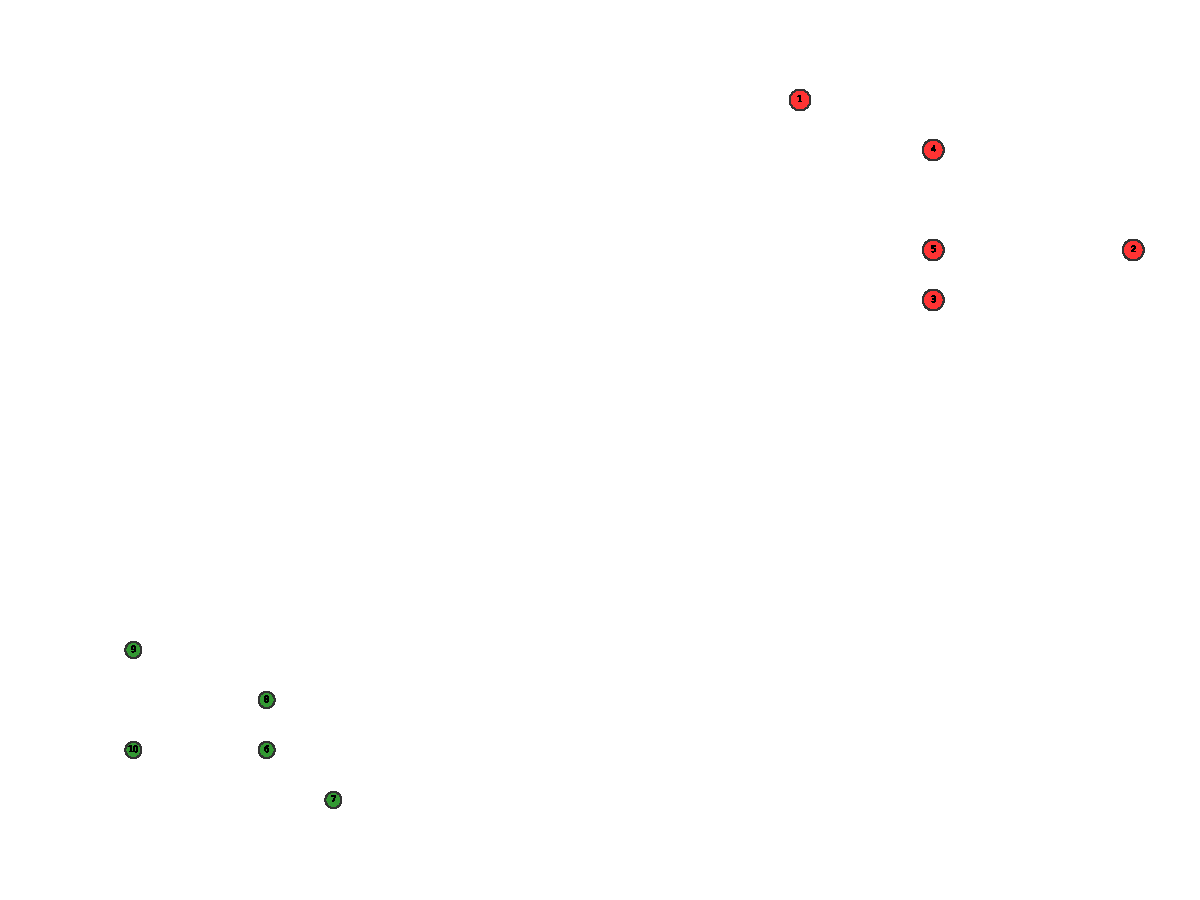
\includegraphics[scale=0.4]{imagenes/test1.pdf}
    \caption{Pokeparadas distantes de los nodos}
    \label{fig:ej2_caso1}
  \end{center}
\end{figure}


\newpage

La solución óptima obtenida sobre esta instancia devuelve un camino con distancia 78.8592.
Ahora bien, cuando la corremos con la heuristica obtenemos un camino con distancia 104.98, lo que da como diferencia 26.1208.

\begin{figure}[H]
\centering
\begin{minipage}{0.45\textwidth}
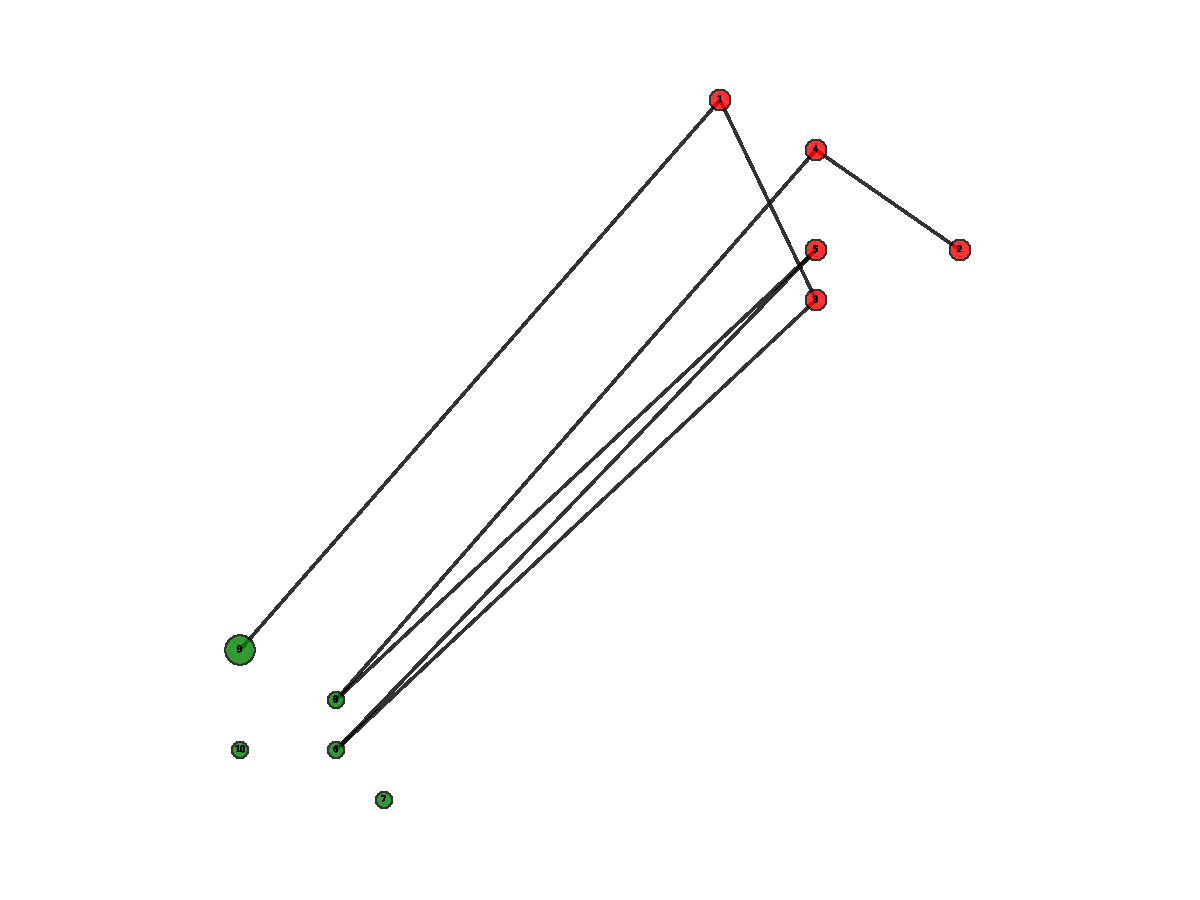
\includegraphics[width=0.9\textwidth]{imagenes/test1-soltest1BT.pdf}
\caption{Solución óptima}
\label{fig:ej2_caso1bt}
\end{minipage}
\qquad
\begin{minipage}{0.45\textwidth}
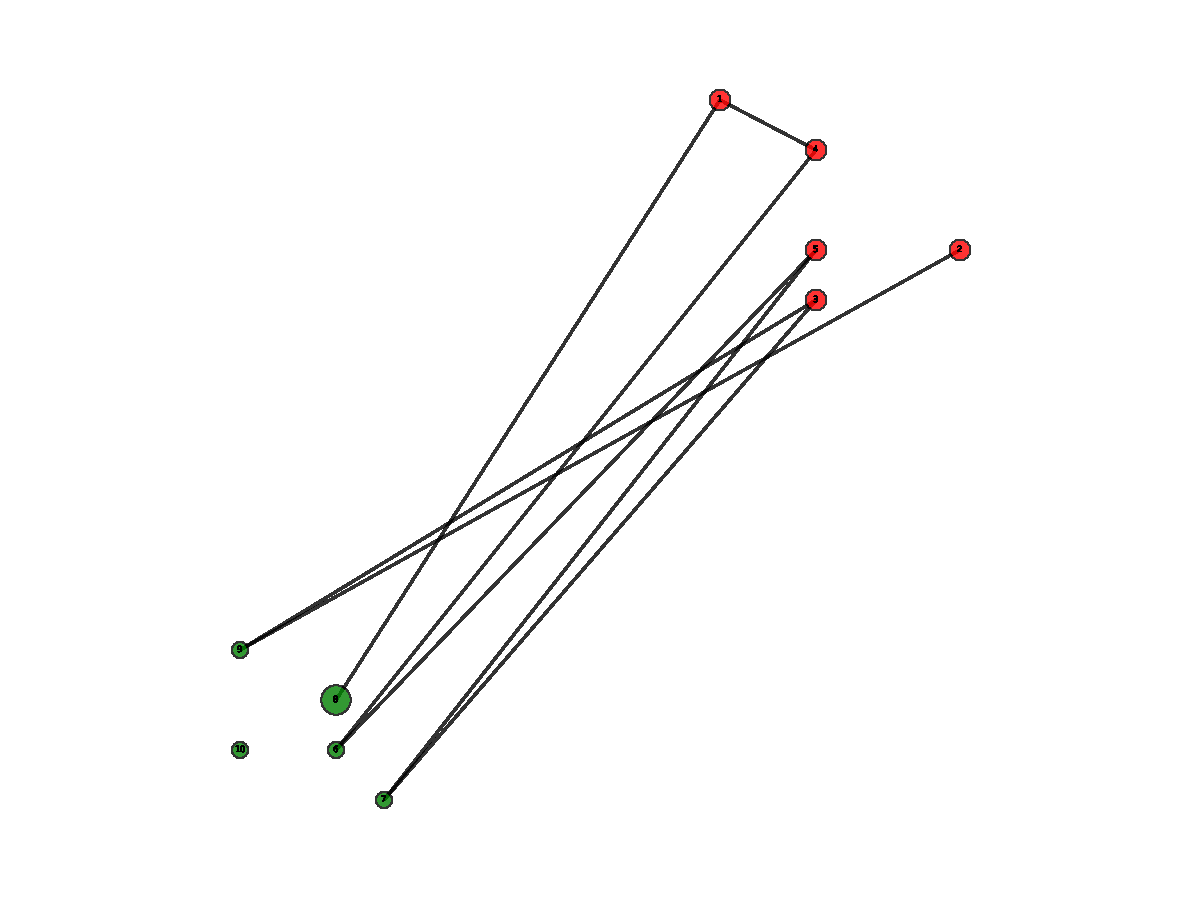
\includegraphics[width=0.9\textwidth]{imagenes/test1-soltest1H.pdf}
\caption{Solución con heuristica}
\label{fig:ej2_caso1h}
\end{minipage}
\end{figure}


Se puede apreciar en las figuras como la heuristica pasa por una poke parada más que en el óptimo y esto hace que la distancia recorrida sea mayor.


\subsubsection{Caso: Pokeparadas y gimnasios de a pares en el plano}

\begin{figure}[H]
  \begin{center}
    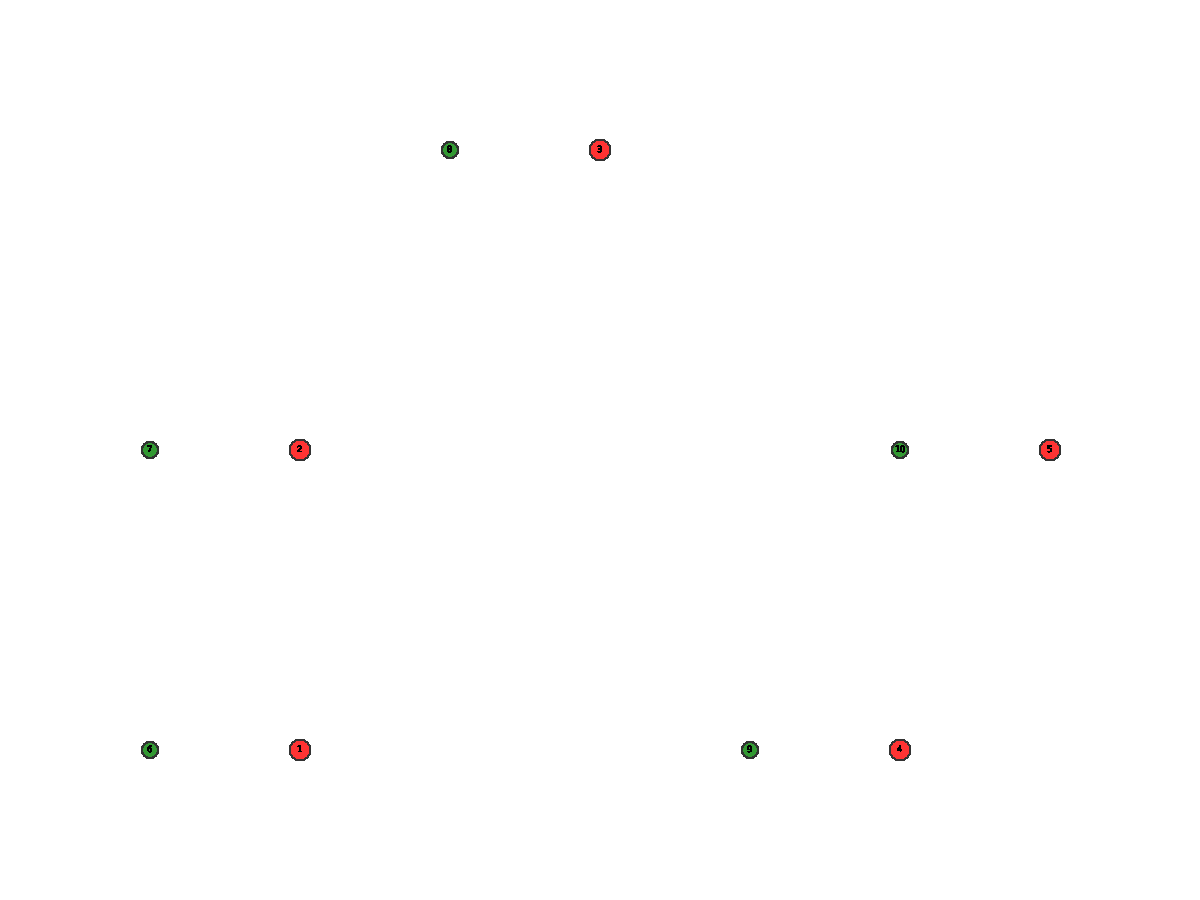
\includegraphics[scale=0.4]{imagenes/test2.pdf}
    \caption{Pokeparadas y Gimnasios de a pares}
    \label{fig:ej2_caso2}
  \end{center}
\end{figure}

En este caso, tenemos 5 gimnasios y 5 pokeparadas que se encuentran de a pares en el plano. Las pociones de los gimnasios tienen valores entre 1 y 3; y la mochila tiene 5 de capacidad.


\begin{figure}[H]
\centering
\begin{minipage}{0.45\textwidth}
\centering
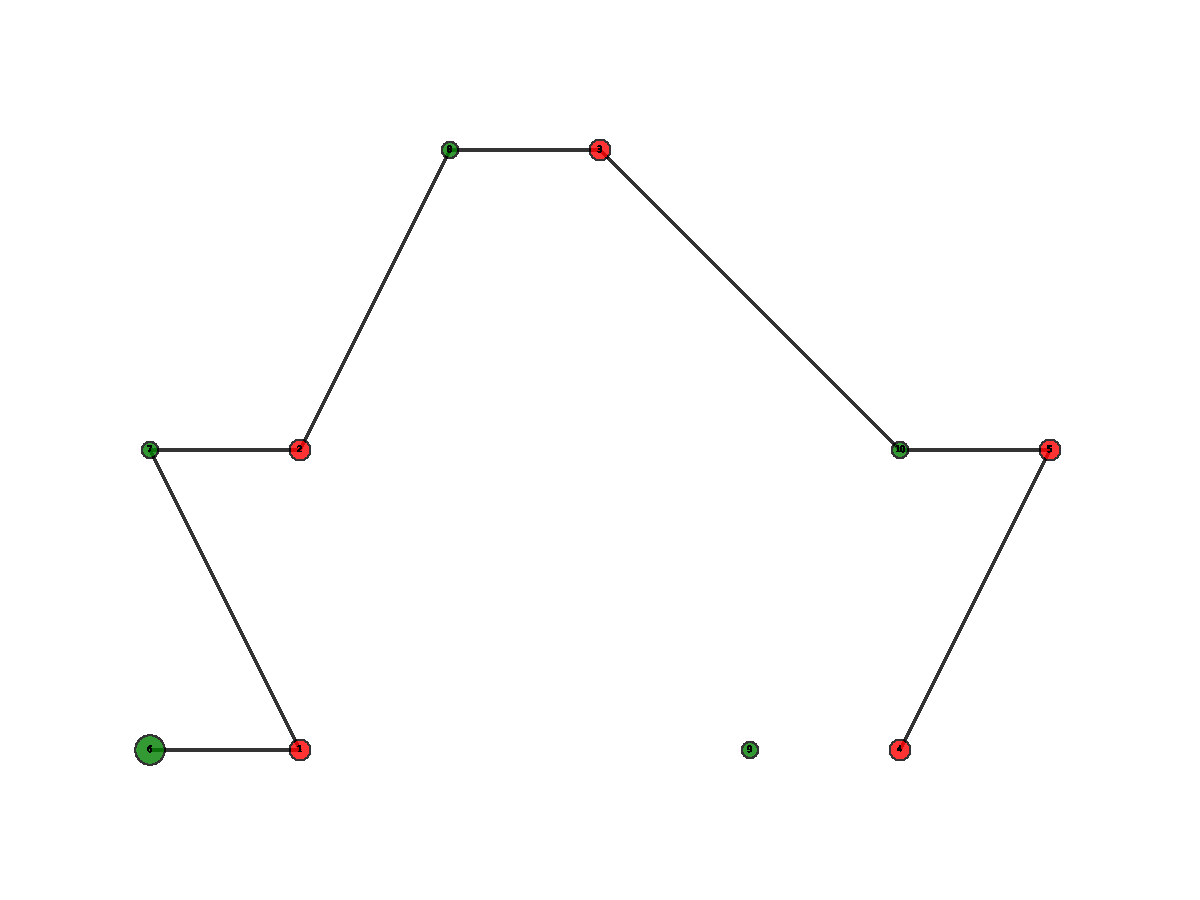
\includegraphics[width=0.9\textwidth]{imagenes/test2-soltest2BT.pdf}
\caption{Solución óptima}
\label{fig:ej2_caso2bt}
\end{minipage}
\qquad
\begin{minipage}{0.45\textwidth}
\centering
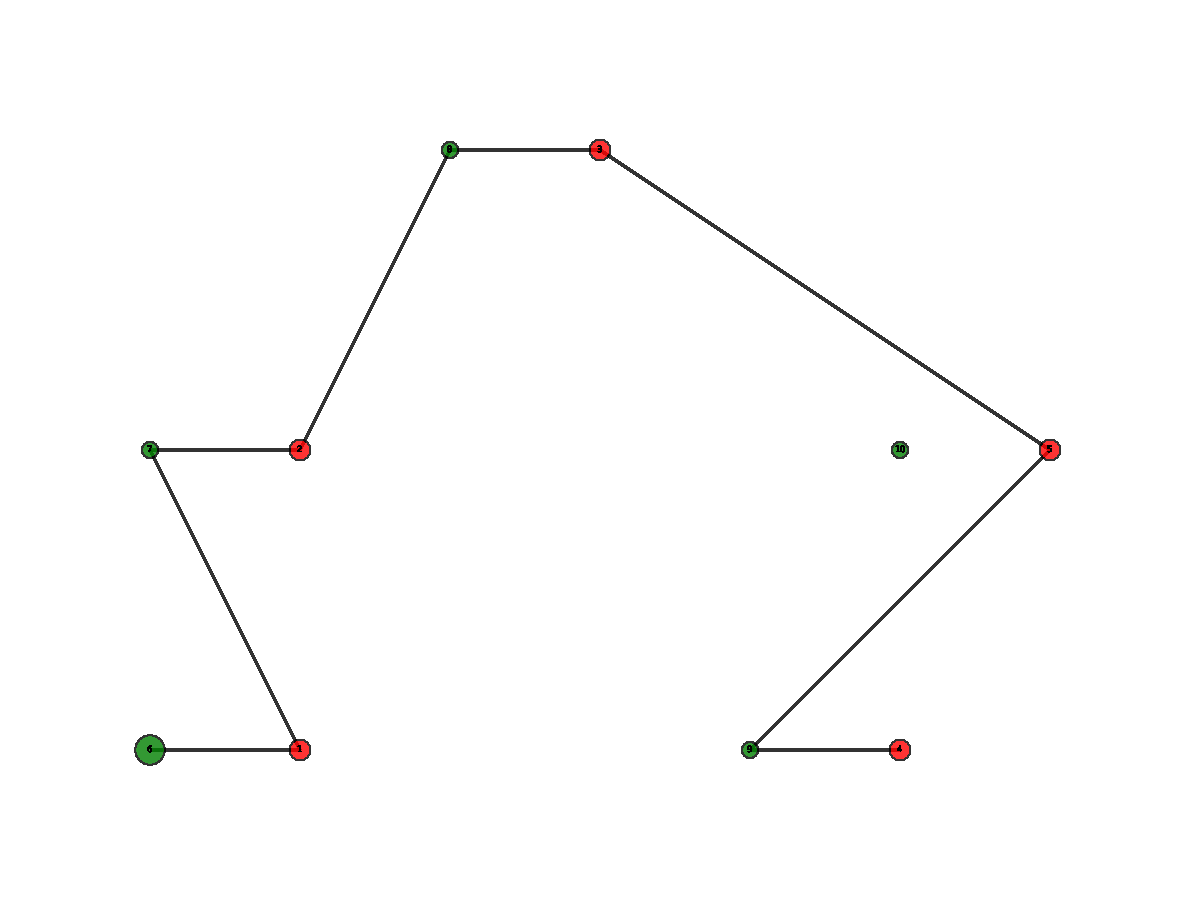
\includegraphics[width=0.9\textwidth]{imagenes/test2-soltest2H.pdf}
\caption{Solución con heuristica}
\label{fig:ej2_caso2h}
\end{minipage}
\end{figure}

La solución óptima devuelve un camino con distancia total 13.5366, en cambio la heuristica devuelve un camino con distancia 14.9061. La diferencia es de 1.3695.



Tiene sentido que para este caso tenga una diferencia chica la una de la otra ya que por como están dispuestas las pokeparadas y los gimnasios y, dado que la heuristica primero genera un camino de gimnasios, en estos casos va a haber una diferencia de distancias pequeña.


\subsubsection{Caso: Sólo gimnasios}

\begin{figure}[H]
  \begin{center}
    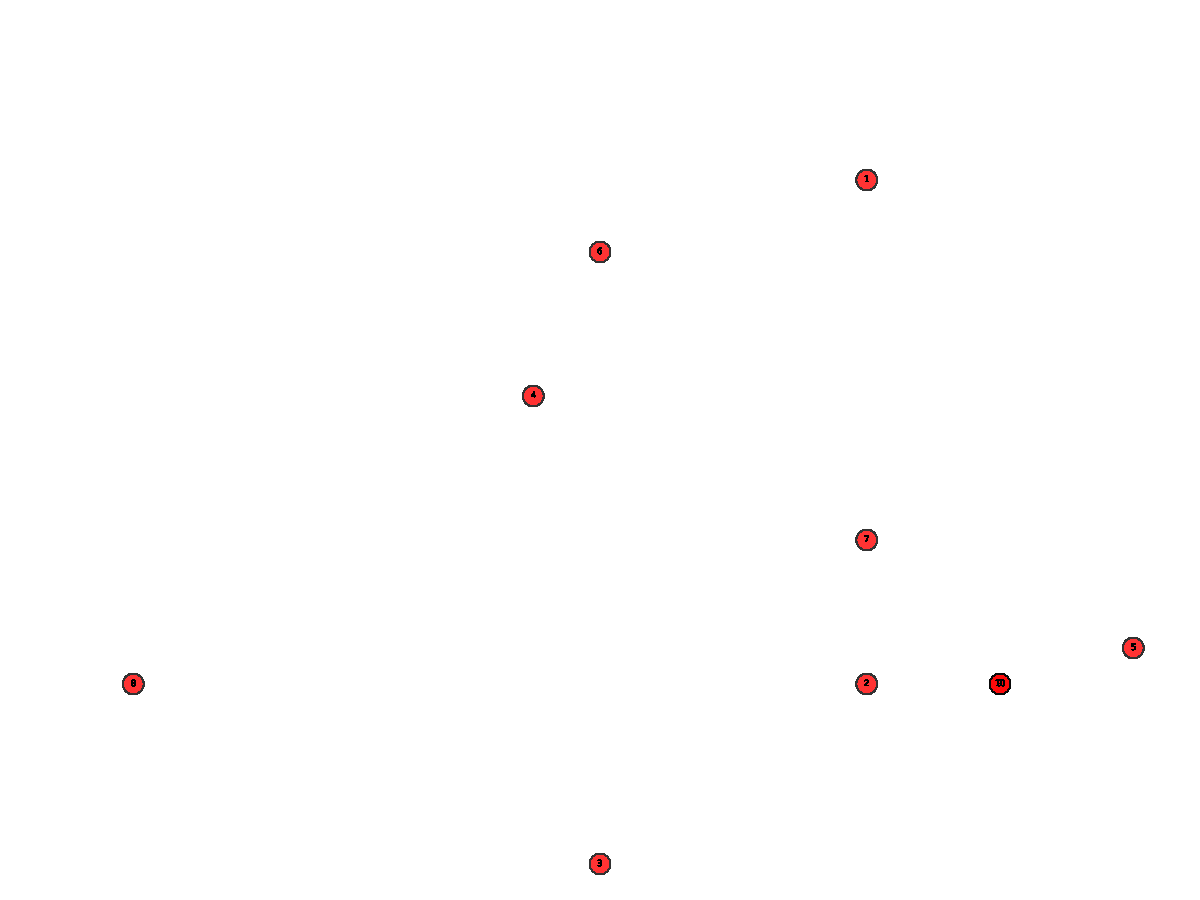
\includegraphics[scale=0.4]{imagenes/test3.pdf}
    \caption{Sólo Gimnasios}
    \label{fig:ej2_caso3}
  \end{center}
\end{figure}

Este caso sólo presenta 10 gimnasios a los que no necesitan pociones para ser vencidos (en cada uno el valor necesario es cero). Éstos poséen posiciones aleatorias dentro del mapa.

Cómo la heuristica genera un camino de gimnasios veamos como se comporta en este caso contra la solución óptima.

\begin{figure}[H]
\centering
\begin{minipage}{0.45\textwidth}
\centering
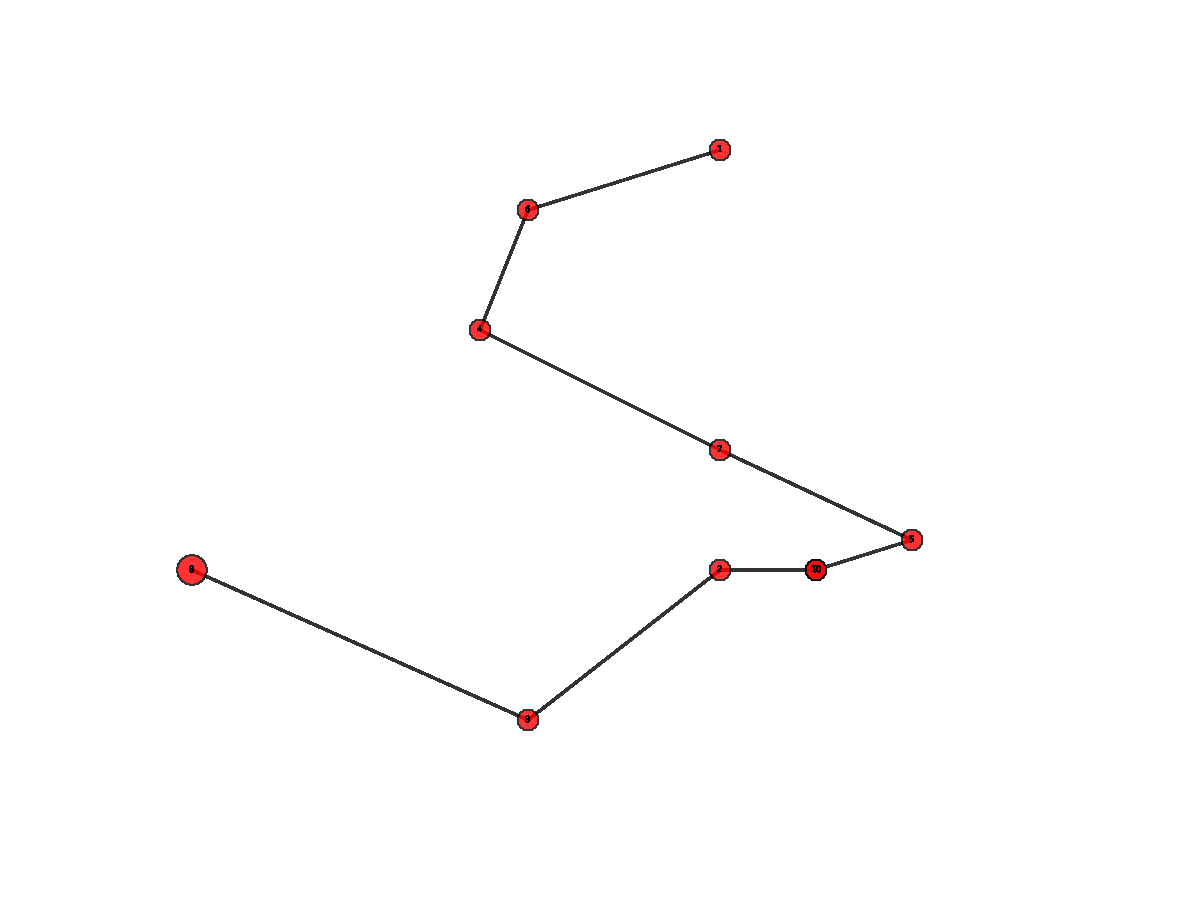
\includegraphics[width=0.9\textwidth]{imagenes/test3-soltest3BT.pdf}
\caption{Solución óptima}
\label{fig:ej2_caso3bt}
\end{minipage}
\qquad
\begin{minipage}{0.45\textwidth}
\centering
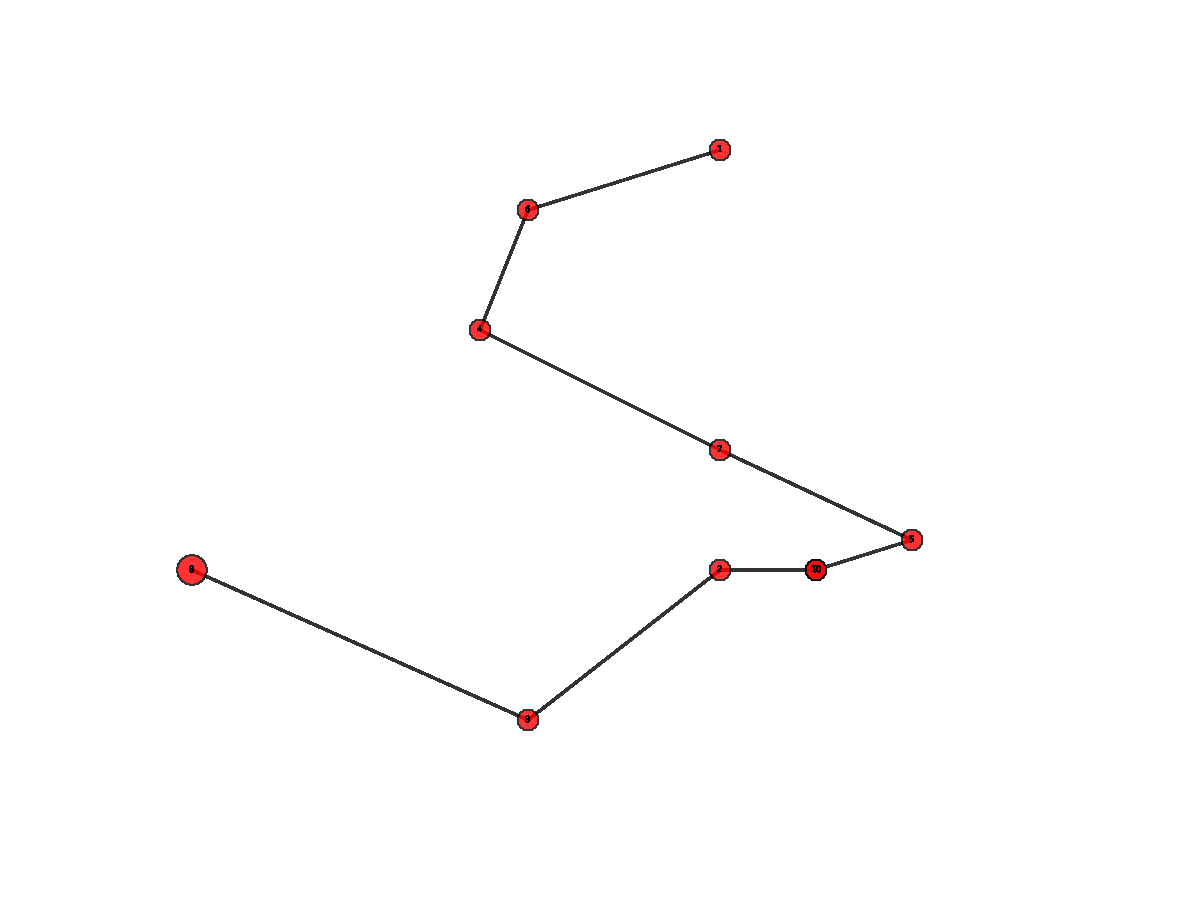
\includegraphics[width=0.9\textwidth]{imagenes/test3-soltest3H.pdf}
\caption{Solución con heuristica}
\label{fig:ej2_caso3h}
\end{minipage}
\end{figure}

Tanto la solución óptima como la heuristica en este caso devolvieron el mismo camino. Ésto nos dice que podemos obtener mejores casos cuando se tienen más gimnasios que paradas y las instancias tienen solución.


\subsubsection{Caso: Posiciones aleatorias}

\begin{figure}[H]
  \begin{center}
    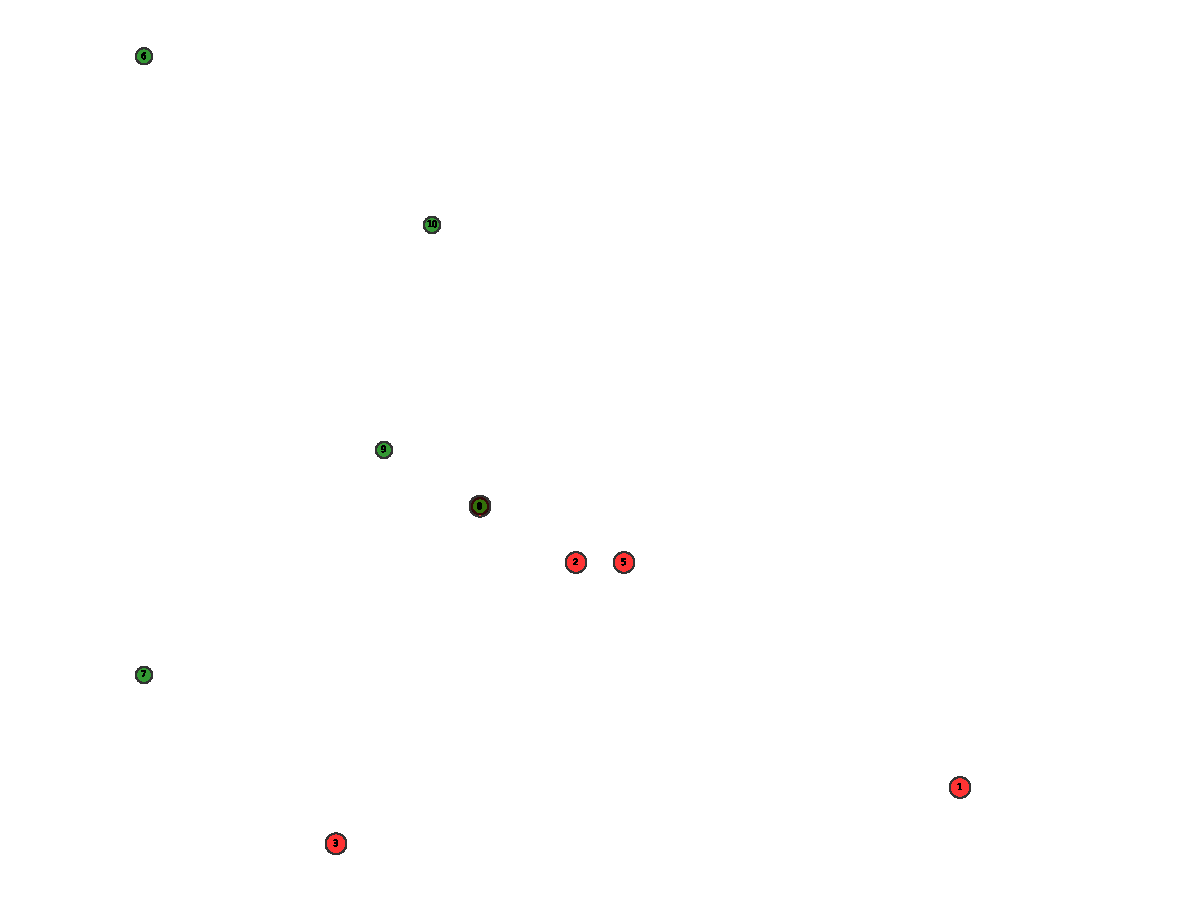
\includegraphics[scale=0.4]{imagenes/test4.pdf}
    \caption{Gimnasios y Paradas con posiciones aleatorias}
    \label{fig:ej2_caso4}
  \end{center}
\end{figure}

En este caso tenemos 5 gimnasios y 5 pokeparadas dispersos en el plano. Se cuenta con una mochila de tamaño 3 y cada gimnasio necesita 3 pociones para ser vencido.

\begin{figure}[H]
\centering
\begin{minipage}{0.45\textwidth}
\centering
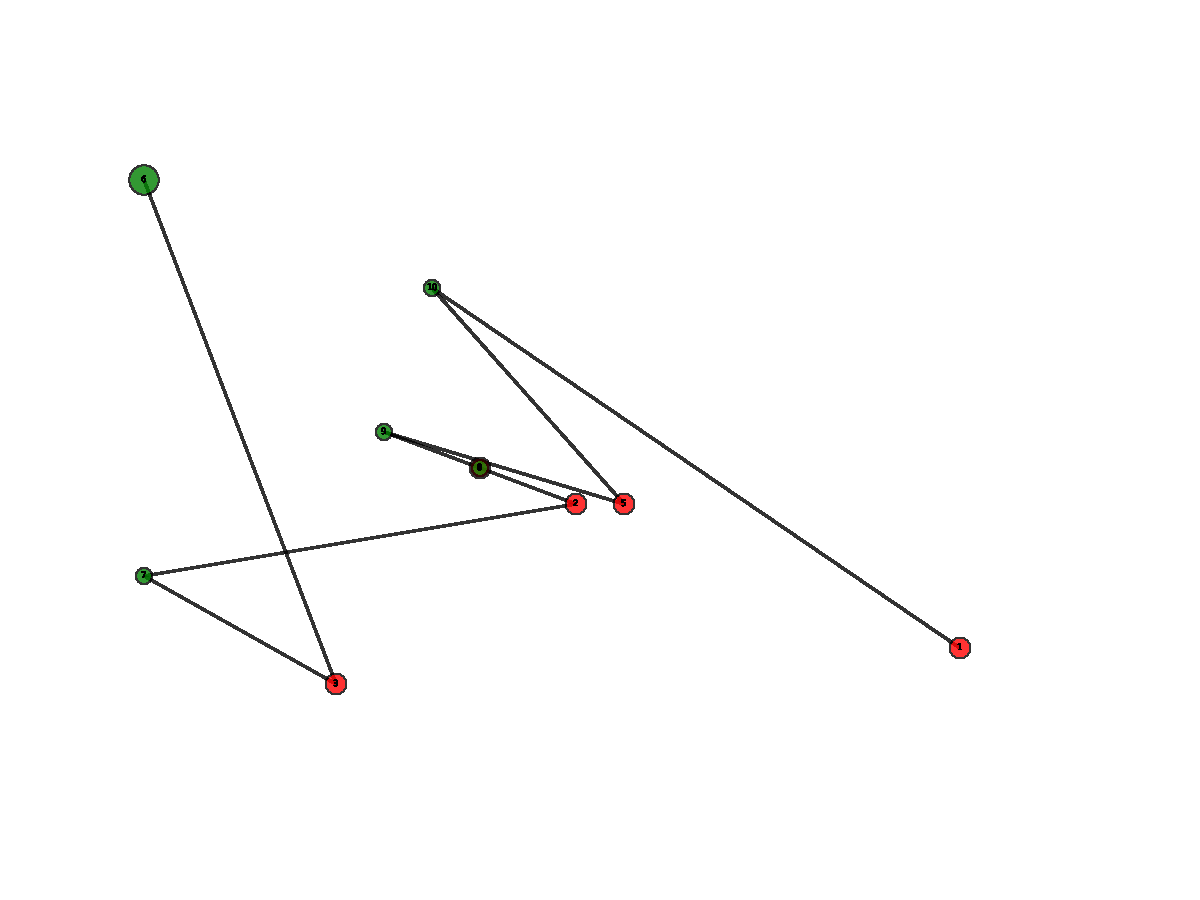
\includegraphics[width=0.9\textwidth]{imagenes/test4-soltest4BT.pdf}
\caption{Solución óptima}
\label{fig:ej2_caso4bt}
\end{minipage}
\qquad
\begin{minipage}{0.45\textwidth}
\centering
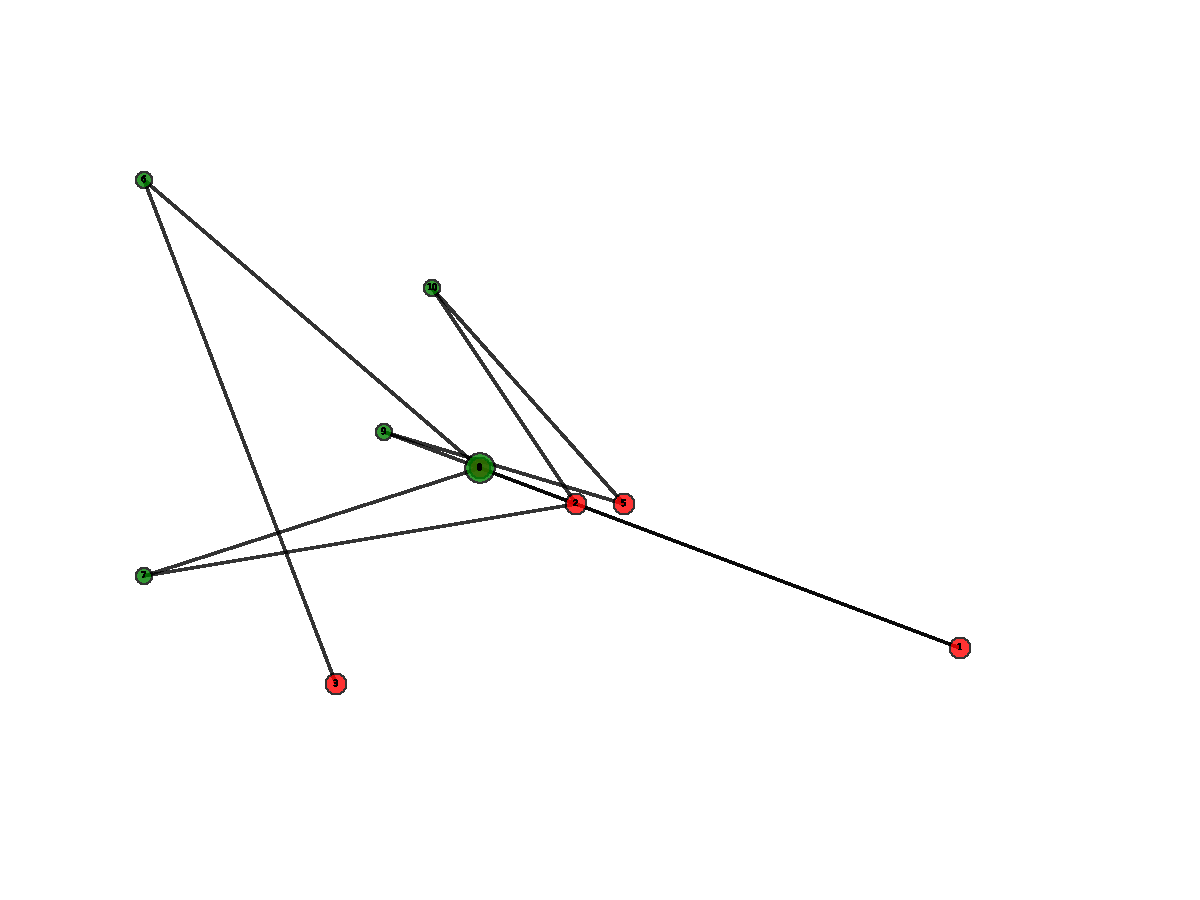
\includegraphics[width=0.9\textwidth]{imagenes/test4-soltest4H.pdf}
\caption{Solución con heuristica}
\label{fig:ej2_caso4h}
\end{minipage}
\end{figure}

La solución óptima obtenida para esta instancia devuelve un camino con distancia recorrida 60.7142, mientras que la heuristica devuelve un camino con distancia 85.9269. La diferencia entre distancias es de 25.2127. Esto nos dice que para grafos aleatorios podemos obtener casos muy lejanos de la solución óptima.

\subsubsection{Caso: La heuristica no encuentra una solución}

Los peores casos de la heuristica son los que no encuentra una solución cuando la hay. Este es uno de esos casos.

\begin{figure}[H]
  \begin{center}
    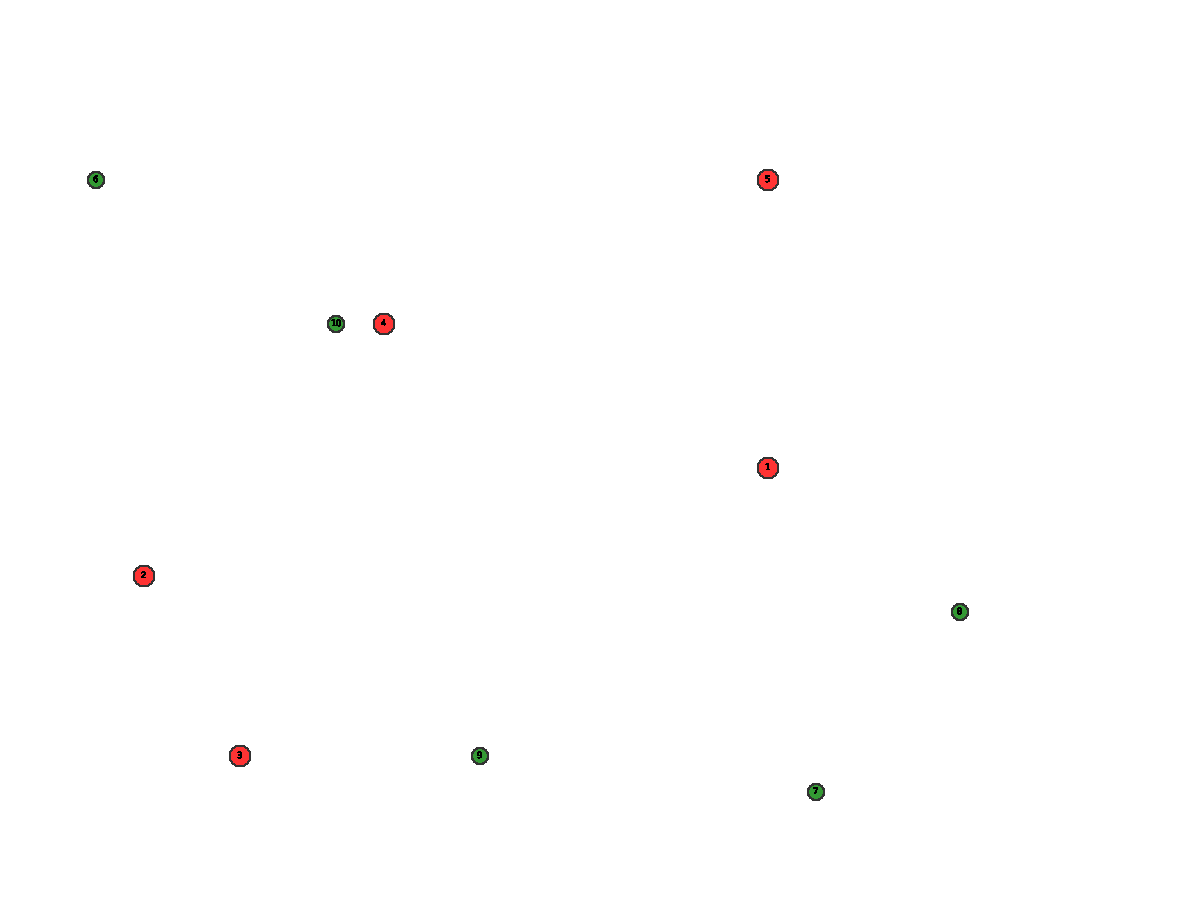
\includegraphics[scale=0.4]{imagenes/test5.pdf}
    \caption{Grafo en el que nuestra heuristica no encuentra solución pero la tiene.}
    \label{fig:ej2_caso4}
  \end{center}
\end{figure}

La cantidad de gimnasios y de paradas es de 5, la mochila tiene capacidad 5 y los gimnasios piden cantidad de pociones entre 1 y 5 para poder vencerlos.

La solución óptima es la siguiente:

\begin{figure}[H]
  \begin{center}
    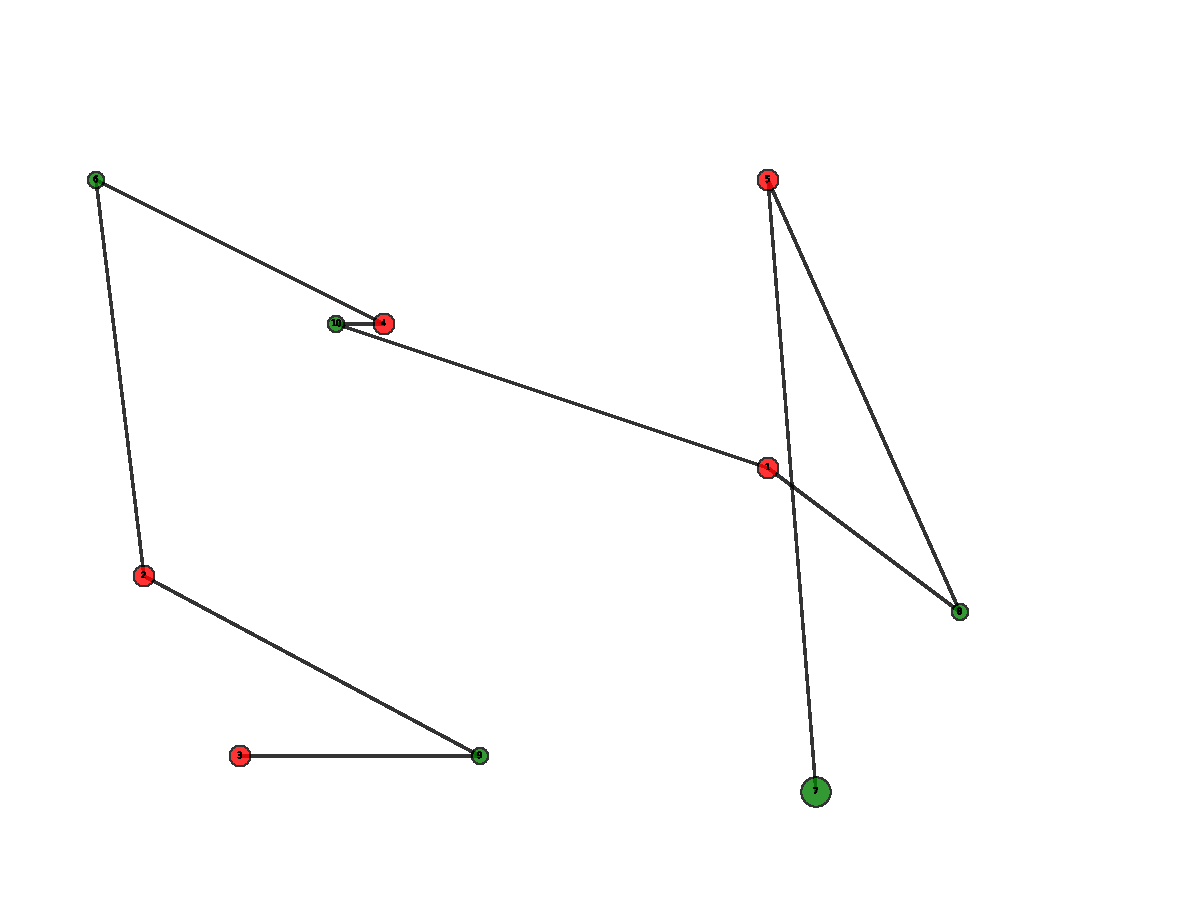
\includegraphics[scale=0.4]{imagenes/test5-soltest5BT.pdf}
    \caption{Solución óptima.}
    \label{fig:ej2_caso4}
  \end{center}
\end{figure}


\subsection{Experimentación}

Con el fin de observar la performance del algoritmo en términos de tiempo de ejecución en función del tamaño de entrada, generamos...